%-----------------------------------------------------------------------
% Beginning of chap2.tex
%-----------------------------------------------------------------------
%
%  AMS-LaTeX sample file for a chapter of a monograph, to be used with
%  an AMS monograph document class.  This is a data file input by
%  chapter.tex.
%
%  Use this file as a model for a chapter; DO NOT START BY removing its
%  contents and filling in your own text.
% 
%%%%%%%%%%%%%%%%%%%%%%%%%%%%%%%%%%%%%%%%%%%%%%%%%%%%%%%%%%%%%%%%%%%%%%%%


\chapter*{Lecture 4}
\addcontentsline{toc}{chapter}{Lecture 4}
\addtocounter{chapter}{4}
\addtocounter{section}{0}
\numberwithin{theorem}{chapter}
%\numberwithin{section}{chapter}
\numberwithin{equation}{chapter}

% \epigraph{}{--- \textup{}}

Iterative algorithms for solving a problem of the form
\begin{equation}\label{eq:min}
 \minimize f(\vct{x})
\end{equation}
on $\R^n$ generate a sequence of vectors $\vct{x}_0,\vct{x}_1,\dots$ in the hope that this sequence converges to a (local or global) minimizer $\vct{x}^*$ of~\eqref{eq:min}. In this lecture we first study step length selection procedures and then study what it means for a sequence to converge, and how to quantify the speed of convergence.

\section{Step length selection}\label{sec:steplength}
When moving in a descent direction $\vct{p}_k$ (not necessarily the steepest descent direction), 
\begin{equation*}
  \vct{x}_{k+1} = \vct{x}_k+\alpha_k \vct{p}_k
\end{equation*}
we can only guarantee that the function value will decrease if the step length $\alpha_k$ is small enough. If we move too far in a descent direction, we might even land at a point where $f$ is larger than where we started! It is therefore important to choose a step length that 
\begin{itemize}
\item is not too small (so that the algorithm does not take too long);
\item is not too large (so that we don't end up at a point with larger function value);
\item is easy to compute.
\end{itemize} 

An optimal step $\alpha$ for a descent method would be the minimizer of the function
\begin{equation*}
 \alpha \mapsto \oldphi(\alpha) := f(\vct{x}_k+\alpha \vct{p}_k).
\end{equation*}
In practice, minimizing this function is not always the most efficient thing to do (or even possible). One would rather choose a step length that satisfies some criteria that ensure that the sequence $\vct{x}_k$ converges to a minimizer $\vct{x}^*$ under suitable conditions on a function $f$. One such condition is a \textbf{sufficient decrease condition},
\begin{equation*}
 f(\vct{x}_k+\alpha \vct{p}_k) \leq f(\vct{x}_k) + c \alpha\ip{\nabla f(\vct{x}_k)}{\vct{p}_k} =: \ell(\alpha),
\end{equation*}
with $c\in (0,1)$. Note that $\oldphi'(0) = \ip{\nabla f(\vct{x}_k)}{\vct{p}_k} <0$, because $\vct{p}_k$ is a descent direction. The function $\ell(\alpha)$ is therefore a line through $f(\vct{x}_k)$ with a slope $c \ip{\nabla f(\vct{x}_k)}{\vct{p}_k} = c\oldphi'(0)>\oldphi'(0)$. To see why this condition is necessary, consider the function $f(x)=x^2-1$ and the sequence $x_k = \sqrt{1+1/k}$ for $k\geq 1$. Clearly, the sequence $f(\vct{x}_k)=1/k$ decreases, but fails to converge to the minimizer $f(0)=-1$.

\begin{figure}[h!]
\centering
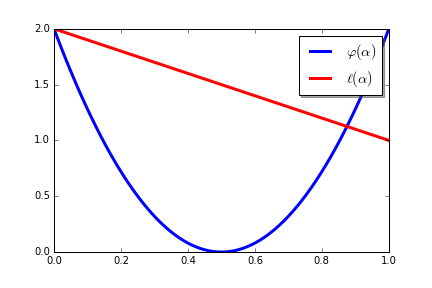
\includegraphics[width=0.6\textwidth]{images/armillo.png}
\caption{The sufficient decrease condition}
\end{figure}

The sufficient decrease condition (also called Armijo condition) can always be satisfied if $\alpha$ is chosen small enough, but the algorithm may become very slow. It is therefore common to supplement the sufficient descent condition with other criteria that guarantee that sufficient progress is made. Two of the commonly used criteria are:

\begin{itemize}
\item the Wolfe conditions, which add a {\em curvature condition}
\begin{equation*}
\oldphi'(\alpha)\geq \tilde{c} \oldphi'(0)
\end{equation*}
for some $\tilde{c}\in (c,1)$, which gives a lower bound on the slope of the new point;
\item the Armijo-Goldstein conditions, which state that a step length $\alpha_k$ should additionally satisfy bound 
\begin{equation}\label{eq:armgold}
  f(\vct{x}_k)+(1-c)\alpha_k \ip{\nabla f(\vct{x}_k)}{\vct{p}_k} \leq f(\vct{x}_k+\alpha_k \vct{p}_k),
\end{equation}
which gives a lower bound on the step size.
\end{itemize}

Another common approach is \textbf{backtracking}: in this method one uses a high initial value of $\alpha$ (for example, $\alpha=1$), and then decreases it until the sufficient descent condition is satisfied. 

\begin{example}
 Consider the function $f\colon \R^2\to \R$ defined by $f(\vct{x}) = x_1^2+x_2^2$. The gradient is $\nabla f(\vct{x}) = 2\vct{x}$, and the $\phi$ function at $\vct{x}_k=(1,1)^{\trans}$
 \begin{equation*}
  \phi(\alpha) = f(\vct{x}_k-\alpha \nabla f(\vct{x}_k)) = 2(1-2\alpha)^2, \quad \phi'(\alpha) = -8(1-2\alpha).
 \end{equation*}
The Armijo-Goldstein conditions~\eqref{eq:armgold} then state that we can choose $\alpha$ such that
\begin{equation*}
 2(1-4(1-c)\alpha) \leq 2(1-2\alpha)^2 \leq 2(1-4c\alpha).
\end{equation*}
The optimal step length in this case would be $\alpha=0.5$.
\end{example}

\section{Convergence of iterative methods}
A sequence of vectors $\{\vct{x}_k\}$ in $\R^n$, $k\geq 0$, {\em converges} to a vector $\vct{x}^*$ with respect to a norm $\norm{\cdot}$ as $k\to \infty$, written $\vct{x}_k\to \vct{x}$, if the sequence of numbers $\norm{\vct{x}_k-\vct{x}^*}$ converges to zero. More formally, if for every $\e>0$ there exists an index $N$ such that for all $n\geq N$,
\begin{equation*}
 \norm{\vct{x}_n-\vct{x}^*}< \e.
\end{equation*}
Iterative algorithms will rarely find the exact solution to a problem like~\eqref{eq:min}, so we will usually be happy to find a solution that differs from the true one by at most some specified accuracy.

\begin{definition}
 A sequence of vectors $\{\vct{x}_k\}$, $k\geq 0$, is said to converge to $\vct{x}^*$ 
 \begin{itemize}
 \item[(a)] linearly (or Q-linear, Q for quotient), if there exist an $r\in (0,1)$ such that for sufficiently large $k$,
 \begin{equation*}
  \norm{\vct{x}_{k+1}-\vct{x}^*}\leq r\norm{\vct{x}_k-\vct{x}^*}.
 \end{equation*}
 \item[(b)] superlinearly, if 
 \begin{equation*}
 \lim_{k\to \infty} \frac{\norm{\vct{x}_{k+1}-\vct{x}^*}}{\norm{\vct{x}_k-\vct{x}^*}} = 0,
 \end{equation*}
 \item[(c)] with order $p$, if there exists a constant $M>0$, such that for sufficiently large $k$,
 \begin{equation*}
  \norm{\vct{x}_{k+1}-\vct{x}^*}\leq M\norm{\vct{x}_k-\vct{x}^*}^p.
 \end{equation*}
The case $p=2$ is called {\em quadratic convergence}.
 \end{itemize}
\end{definition}

Of course, as mentioned earlier, these definitions depend on the choice of a norm. It can be shown that quadratic convergence implies superlinear convergence, and superlinear convergence implies linear convergence.

\begin{example}
 Consider the sequence of numbers $x_k = 1/2^{r^k}$ for some $r>1$. Clearly, $x_k\to x^*=0$ as $k\to \infty$. Moreover,
 \begin{equation*}
  x_{k+1}=\frac{1}{2^{r^{k+1}}}=\frac{1}{2^{r^{k}r}}=\left(\frac{1}{2^{r^{k}}}\right)^r=x_k^r,
 \end{equation*}
which shows that the sequence has rate of convergence $r$.
\end{example}

\section{Convergence of gradient descent}
In this section, a norm $\norm{\cdot}$ will refere to the $2$-norm, unless otherwise stated.
We now study the convergence of gradient descent for the least squares problem
\begin{equation}\label{eq:ffromgraddesc}
 \minimize f(\vct{x}) = \frac{1}{2}\norm{\mtx{A}\vct{x}-\vct{b}}^2,
\end{equation}
where $\mtx{A}\in \R^{m\times n}$ with $m\geq n$ of full rank.
As we have seen in Lecture 3, the gradient descent method is the procedure
\begin{equation*}
 \vct{x}_{k+1}=\vct{x}_{k} + \alpha_k\vct{r}_k,
\end{equation*}
where the step length and the {\em residual} are given by
\begin{equation*}
 \alpha_k = \frac{\norm{\vct{r}_k}^2}{\norm{\mtx{A}\vct{r}_k}^2}, \quad \vct{r}_k = \mtx{A}^{\trans}(\vct{b}-\mtx{A}\vct{x}_k)=-\nabla f(\vct{x}_k).
\end{equation*}
At the minimizer, the residual is 
\begin{equation}\label{eq:reszero}
 \vct{r} = -\nabla f(\vct{x}^*)=\mtx{A}^{\trans}(\vct{b}-\mtx{A}\vct{x}^*) = 0,
\end{equation}
and 
as the sequence $\vct{x}_k$ converges to $\vct{x}^*$, the norms of the residuals converge to $0$. Conversely, the residual is related to the difference $\vct{x}_k-\vct{x}^*$ by
\begin{equation}\label{eq:resdif}
 \vct{r}_k = \mtx{A}^{\trans}(\vct{b}-\mtx{A}\vct{x}_k) = \mtx{A}^{\trans}(\vct{b}-\mtx{A}\vct{x}_k-(\vct{b}-\mtx{A}\vct{x}^*)) = \mtx{A}^{\trans}\mtx{A}(\vct{x_k}-\vct{x}^*),
\end{equation}
where we used the ``intelligent zero'' ~\eqref{eq:reszero}. Therefore
\begin{equation*}
 \norm{\vct{x}_k-\vct{x}^*} = \norm{(\mtx{A}^{\trans}\mtx{A})^{-1}\vct{r}}\leq \norm{(\mtx{A}^{\trans}\mtx{A})^{-1}}\norm{\vct{r}_k},
\end{equation*}
where $\norm{\mtx{B}} = \max_{\vct{x}\neq \zerovct}\norm{\mtx{B}\vct{x}}/\norm{\vct{x}}$ is the operator norm of a matrix $\mtx{B}$ with respect to the $2$-norm. Consequently, if the sequence $\norm{\vct{r}_k}$ converges to zero, so does the sequence $\norm{\vct{x}_k-\vct{x}^*}$. A reasonable criterium is to stop the algorithm is therefore when the residual norm $\norm{\vct{r}_k}$ is below a predefined tolerance $\e$. 

%For the following, we use the norm
%\begin{equation*}
% \norm{\vct{x}}_{\mtx{A}}^2 := \ip{\mtx{A}\vct{x}}{\mtx{A}\vct{x}} = \norm{\mtx{A}\vct{x}}^2.
%\end{equation*}
%We have the bounds
%\begin{equation*}
% \norm{\mtx{A}^{\dagger}}^{-1} \norm{\vct{x}} \leq \norm{\vct{x}}_{\mtx{A}} \leq \norm{\mtx{A}} \norm{\vct{x}},
%\end{equation*}
%where $\mtx{A}^{\dagger}=(\mtx{A}^{\trans}\mtx{A})^{-1}\mtx{A}^{\trans}$ is the {\em Moore-Penrose pseudoinverse} of $\mtx{A}$. The important consequence of these inequalities is that convergence with respect to the $\norm{\cdot}_{\mtx{A}}$ norm is equivalent to convergence with respect to the $2$-norm.
%
%A simple but nevertheless very useful observation is the following.
%\begin{lemma}\label{le:anorm}
% The difference between the function value at some $\vct{x}\in \R^n$ and the optimal value is
% \begin{equation*}
%  f(\vct{x})-f(\vct{x}^*) = \frac{1}{2}\norm{\vct{x}-\vct{x}^*}_{\mtx{A}}^2.
% \end{equation*}
%\end{lemma}
%
%\begin{proof}
% This proceeds by straight-forward calculation:
% \begin{align*}
%  f(\vct{x}^*)-f(\vct{x})+\frac{1}{2}\norm{\vct{x}-\vct{x}^*}_{\mtx{A}}^2 &= \frac{1}{2}\norm{\mtx{A}\vct{x}^*-b}^2-\frac{1}{2}\norm{\mtx{A}\vct{x}-\vct{b}}^2+\frac{1}{2}\norm{\mtx{A}(\vct{x}-\vct{x}^*)}^2\\
%  &= \frac{1}{2}\norm{\mtx{A}\vct{x}^*-\vct{b}}^2-\frac{1}{2}\norm{\mtx{A}\vct{x}-\vct{b}}^2+\frac{1}{2}\norm{\mtx{A}\vct{x}-\vct{b}-(\mtx{A}\vct{x}^*-\vct{b})}^2\\
%  &= \norm{\mtx{A}\vct{x}^*-\vct{b}}^2 - \ip{\mtx{A}\vct{x}^*-\vct{b}}{(\mtx{A}\vct{x}-\vct{b})}\\
%  &= \ip{\mtx{A}\vct{x}^*-\vct{b}}{\mtx{A}\vct{x}^*-\vct{b}-(\mtx{A}\vct{x}-\vct{b})}\\
%  &= \ip{\mtx{A}\vct{x}^*-\vct{b}}{\mtx{A}(\vct{x}^*-\vct{x})}\\
%  &= \ip{\mtx{A}^{\trans}(\mtx{A}\vct{x}^*-\vct{b})}{\vct{x}^*-\vct{x}} = \ip{\nabla f(\vct{x}^*)}{\vct{x}^*-\vct{x}} = 0,
% \end{align*}
% where the last equality follows from~\eqref{eq:reszero}.
%\end{proof}
%
%
%
%
%We first derive a bound on the decrease of the function value at each step.
%
%\begin{lemma}\label{le:41}
% For the function $f$ as in~\eqref{eq:ffromgraddesc},
% \begin{equation*}
%  f(\vct{x}_k)-f(\vct{x}_{k+1}) =  \frac{1}{2}\frac{\norm{\vct{r}_k}^4}{\norm{\mtx{A}\vct{r}_k}^2}\geq \frac{1}{2}\frac{\norm{\vct{r}_k}^2}{\norm{\mtx{A}}^2},
% \end{equation*}
%where $\norm{\mtx{A}} := \max_{\vct{x}\neq \zerovct} \norm{\mtx{A}\vct{x}}/\norm{\vct{x}}$ is the {\em operator norm} of $\mtx{A}$ with respect to the $2$-norm.
%\end{lemma}
%
%\begin{proof} Using the identity $\norm{\vct{x}}^2=\ip{\vct{x}}{\vct{x}}$ and the bilinearity
% \begin{equation*}
%  \norm{\vct{x}+\vct{y}}^2=\ip{\vct{x}+\vct{y}}{\vct{x}+\vct{y}}=\ip{\vct{x}}{\vct{x}}+2\ip{\vct{x}}{\vct{y}}+\ip{\vct{y}}{\vct{y}} = \norm{\vct{x}}^2+2\ip{\vct{x}}{\vct{y}}+\norm{\vct{y}}^2,
% \end{equation*}
%we compute
% \begin{align}\label{eq:derivation}
% \begin{split}
%  f(\vct{x}_{k+1})=f(\vct{x}_k+\alpha_k\vct{r}_k) &= \frac{1}{2}\norm{\mtx{A}\vct{x}_k+\alpha_k\mtx{A}\vct{r}_k-\vct{b}}^2\\
% &= \frac{1}{2}\norm{\mtx{A}\vct{x}_k-\vct{b}}^2+\ip{\mtx{A}\vct{x}_k-\vct{b}}{\alpha_k \mtx{A}\vct{r}_k}+\frac{1}{2}\alpha_k^2\norm{\mtx{A}\vct{r}_k}^2\\
% &=\frac{1}{2}\norm{\mtx{A}\vct{x}_k-\vct{b}}^2+\alpha_k\ip{\mtx{A}^{\trans}(\mtx{A}\vct{x}_k-\vct{b})}{\vct{r}_k}+\frac{1}{2}\alpha_k^2\norm{\mtx{A}\vct{r}_k}^2\\
%&= f(\vct{x}_k)-\alpha_k \ip{\vct{r}_k}{\vct{r}_k}+\frac{1}{2}\alpha_k^2\norm{\mtx{A}\vct{r}_k}^2.
%  \end{split}
%  \end{align}
%Substituting $\alpha_k=\norm{\vct{r}_k}^2/\norm{\mtx{A}\vct{r}_k}^2$, we get
%\begin{equation*}
% f(\vct{x}_{k+1}) = f(\vct{x}_k) -\frac{\norm{\vct{r}_k}^4}{\norm{\mtx{A}\vct{r}_k}^2}+\frac{1}{2}\frac{\norm{\vct{r}_k}^4}{\norm{\mtx{A}\vct{r}_k}^2} = f(\vct{x}_k)-\frac{1}{2}\frac{\norm{\vct{r}_k}^4}{\norm{\mtx{A}\vct{r}_k}^2}.
%\end{equation*}
%Since 
%\begin{equation*}
% \frac{\norm{\mtx{A}\vct{r}_k}}{\norm{\vct{r}_k}} \leq \max_{\vct{x}\neq \zerovct} \frac{\norm{\mtx{A}\vct{x}}}{\norm{\vct{x}}} = \norm{\mtx{A}},
%\end{equation*}
%we get $\norm{\mtx{A}\vct{r}_k}\leq \norm{\mtx{A}}\norm{\vct{r}_k}$, and applying this to~\eqref{eq:derivation}, the inequality
%\begin{equation*}
% f(\vct{x}_{k+1}) \leq f(\vct{x}_k) - \frac{1}{2}\frac{\norm{\vct{r}_k}^2}{\norm{\mtx{A}}^2}.
%\end{equation*}
%Rearranging the gives the claim.
%\end{proof}
%
%% \begin{proof}[Proof of Theorem~\ref{thm:mainlect4}]
%% For a fixed $N$ we sum up the terms from the right-hand side of the bound in Lemma~\ref{le:41},
%%  \begin{equation}\label{eq:tec1}
%%   \frac{1}{2\norm{\mtx{A}}^2} \sum_{k=0}^N \norm{\vct{r}_k}^2 \leq \sum_{k=0}^{N} (f(\vct{x}_{k+1})-f(\vct{x}_k)) = f(\vct{x}_{N+1})-f(\vct{x}_0) \leq f(\vct{x}_0)-f(\vct{x}^*).
%%  \end{equation}
%% As the right-hand side is a constant, as $N\to \infty$ the infinite sum on the left is bounded, and therefore the individual summands have to converge to zero,
%% \begin{equation*}
%%  \lim_{k\to \infty} \norm{\vct{r}_k}^2=0.
%% \end{equation*}
%% As the residuals converge to zero, the errors $\norm{\vct{x}_k-\vct{x}^*}$ also converge to zero. For the bound, we 
%% combine Lemma~\ref{le:41} and Lemma~\ref{le:anorm},
%% \begin{align*}
%%  \norm{\vct{x}_{k+1}-\vct{x}^*}_A^2-\norm{\vct{x}_{k}-\vct{x}^*}_A^2 &= 2(f(\vct{x}_{k+1})-f(\vct{x}^*)-(f(\vct{x}_k)-f(\vct{x}^*)))\\
%%  &= 2(f(\vct{x}_{k+1})-f(\vct{x}_k)) = \frac{\norm{\vct{r}_k}^4}{\norm{\mtx{A}\vct{r}_k}^2}.
%% \end{align*}
%% Using the relationship~\eqref{eq:resdif}, we get
%% \begin{equation*}
%%  \norm{\mtx{A}^{\dagger}\vct{r}_k}^2 = \norm{\mtx{A}(\vct{x}_k-\vct{x}_0)}^2 = \norm{(\vct{x}_k-\vct{x}_0)}_{\mtx{A}}^2,
%% \end{equation*}
%% so that we can write 
%% \begin{equation*}
%%  \frac{\norm{\vct{r}_k}^4}{\norm{\mtx{A}\vct{r}_k}^2} = \frac{\norm{\vct{r}_k}^4}{\norm{\mtx{A}\vct{r}_k}^2} \frac{\norm{\vct{x}_k-\vct{x}^*}_{\mtx{A}}^2}{\norm{\mtx{A}^{\dagger}\vct{r}_k}^2}. 
%% \end{equation*}
%% Using this this with the previous equality,
%% \begin{equation*}
%%  \norm{\vct{x}_{k+1}-\vct{x}^*}_A^2 = \norm{\vct{x}_{k}-\vct{x}^*}_A^2 +\norm{\vct{x}_{k}-\vct{x}^*}_A^2\left( \frac{\norm{\vct{r}_k}^4}{\norm{\mtx{A}\vct{r}_k}^2 \norm{\mtx{A}^{\dagger}\vct{r}_k}^2}. \right).
%% \end{equation*}
%% This was to be shown.
%% \end{proof}
%
%\begin{proof}[Proof of Theorem~\ref{thm:mainlect4}]
%Let
% \begin{equation*}
% g_N := \min_{0\leq k\leq N} \norm{\vct{r}_k}.
%\end{equation*}
%Then since $(N+1)g_N^2\leq \sum_{k=0}^N \norm{\vct{r}_k}^2$, and using Lemma~\ref{le:41},
%\begin{equation*}
% g_N \leq \sqrt{\frac{1}{N+1}\sum_{k=0}^N \norm{\vct{r}_k}^2} \leq \frac{\sqrt{2}\norm{\mtx{A}}}{\sqrt{N+1}}\sqrt{f(\vct{x}_0)-f(\vct{x}^*)}=\frac{\sqrt{2}\norm{\mtx{A}}}{\sqrt{N+1}}\norm{\vct{x}_0-\vct{x}^*}_{\mtx{A}}.
%\end{equation*}
%We know that $g_N< \e$ if $\sqrt{2\norm{\mtx{A}}^2}\norm{\vct{x}_0-\vct{x}^*}_{\mtx{A}}/\sqrt{N+1}<\e$. Solving the latter for $N$, we get that
%\begin{equation*}
% N> \frac{2\norm{\mtx{A}}^2}{\e^2}\norm{\vct{x}_0-\vct{x}^*}_{\mtx{A}}^2-1.
%\end{equation*}
%will guarantee a residual smaller than $\e$.
%\end{proof}

%We next give a bound on the number of iterations that are guaranteed to bring the residual below a certain value. We then state (without proof) a more precise convergence bound in terms of the condition number, that shows that gradient descent for linear least squares has linear convergence.
%
%\begin{theorem}\label{thm:mainlect4}
%Let $\e>0$ be given and assume
%\begin{equation*}
% N> \frac{2\norm{\mtx{A}}^2}{\e^2}\norm{\vct{x}_0-\vct{x}^*}_{\mtx{A}}^2
%\end{equation*}
%for a starting point $\vct{x}_0$, where $\vct{x}^*$ is the minimizer of $f(\vct{x})=\norm{\mtx{A}\vct{x}-\vct{b}}^2$. If $\{\vct{x}_k\}_{k\geq 0}$ is the sequence of vectors generated by gradient descent for this function, then
%\begin{equation*}
% \min_{0\leq k\leq N} \norm{\vct{r}_k}<\e.
%\end{equation*}
%\end{theorem}

The following theorem (whose proof we omit) shows that the gradient descent method for linear least squares converges linearly with respect to the $\mtx{A}$ norm. The statement involves the {\em condition number} of $\mtx{A}$\footnote{The concept of condition number, introduced by Alan Turing while in Manchester, is one of the most important ideas in numerical analysis, as it is indispensable in studying the performance of numerical algorithms.}. This quantity is defined as
\begin{equation*}
 \kappa(\mtx{A}) = \norm{\mtx{A}}\cdot \norm{\mtx{A}^{\dagger}}.
\end{equation*}

\begin{theorem}
 The error in the $k+1$-th iterate is bounded by
 \begin{equation*}
  \norm{\vct{x}_{k+1}-\vct{x}^*} \leq \left(\frac{\kappa^2(\mtx{A})-1}{\kappa^2(\mtx{A})+1}\right)\norm{\vct{x}_{k}-\vct{x}^*}.
 \end{equation*}
\end{theorem}

In particular, the gradient descent algorithm converges linearly. 

%-----------------------------------------------------------------------
% End of chap1.tex
%-----------------------------------------------------------------------
